\documentclass[12pt, a4paper]{article}
\linespread{1.5}

\usepackage[margin=1in]{geometry} % full-width
\usepackage[T1]{fontenc}

\usepackage[dvipsnames]{xcolor}

% Package for tables
\usepackage{booktabs}
\usepackage{tabularx}
% AMS Packages
\usepackage{amsmath}
\usepackage{amsthm}
\usepackage{amssymb}

% Pacchetto per le colonne
\usepackage{multicol}
\setlength{\columnsep}{1cm}

% Package for glyphs
\usepackage{fontawesome} 

% Unicode
\usepackage[utf8]{inputenc}

\usepackage{hyperref}
\hypersetup{
	unicode,
	colorlinks,
	breaklinks,
    linkcolor = Emerald,
    urlcolor = BlueViolet,
    citecolor = BrickRed,
	pdfauthor = {Alex Costanzino, Xiaowei Wen},
	pdftitle = {Bayesian network model for diagnosis of psychiatric diseases},
	pdfsubject = {Fundamentals of Artificial Intelligence and Knowledge Representation},
}

\usepackage[sorting = ynt]{biblatex} %Imports biblatex package
\addbibresource{refs.bib} %Import the bibliography file

\setlength{\parindent}{0pt} % Elimina rientri

\usepackage{caption}
\usepackage{subcaption}

% Impostazioni per il sottotitolo
\usepackage{titling}
\newcommand{\subtitle}[1]{
  \posttitle{
    \par\end{center}
    \begin{center}\large#1\end{center}
    \vskip0.5em}
    }

\usepackage{graphicx, color}
\graphicspath{{fig/}}

%\usepackage[linesnumbered,ruled,vlined,commentsnumbered]{algorithm2e} % use algorithm2e for typesetting algorithms
\usepackage{algorithm, algpseudocode} % use algorithm and algorithmicx for typesetting algorithms
\usepackage{mathrsfs} % for \mathscr command


% Title and other info
\title{\textbf{VLSI - Very Large Scale Integration}}
\subtitle{Combinatorial Decision Making and Optimization \\ Module 1}

\date{Academic year 2020-2021}

% Authors info
\author{Eric Rossetto \\ 
\href{mailto:eric.rossetto@studio.unibo.it}{\faEnvelopeO~eric.rossetto@studio.unibo.it} \\
\href{https://github.com/Erhtric}{\textbf{\textsc{\faGithub~GitHub}}}
\and Xiaowei Wen \\ 
\href{mailto:marco.costante@studio.unibo.it}{\faEnvelopeO~xiaowei.wen@studio.unibo.it} \\
\href{https://github.com/WenXiaowei}{\textbf{\textsc{\faGithub~GitHub}}}
}



\begin{document}
	\maketitle
	\begin{abstract}
	\normalsize
    VLSI (Very Large Scale Integration) refers to the trend of integrating circuits into silicon chips. A typical example is the smartphone. The modern trend of shrinking transistor sizes, allowing engineers to fit more and more transistors into the same area of silicon, has pushed the integration of more and more functions of cellphone circuitry into a single silicon die (i.e. plate). This enabled the modern cellphone to mature into a powerful tool that shrank from the size of a large brick-sized unit to a device small enough to comfortably carry in a pocket or purse, with a video camera, touchscreen, and other advanced features.
	\end{abstract}
	\clearpage
    \tableofcontents
	
	\clearpage

	\section{Introduction}
\clearpage
    \section{Constraint Satisfaction Programming - CSP}

\subsection{Model Description}

\subsection{Improvments}
	- decomposizioni
	- global constraints
	- symmetry breaking
\subsection{Result analysis}

\clearpage
    \section{Satisfiability modulo theories - SMT}

\clearpage
    \input{04_SAT}
    \section{Results analysis and comparison}
In the following tables, we are going to compare the different versions of the model solving the instances from 10 to 19. When the instance is not successfully solved within 300 seconds, we set the time to \emph{0.00}. 
Compared versions are: 
\begin{itemize}
    \item \emph{CSP 1.0.0}: the base version of the model with only strictly needed constraints;
    \item \emph{CSP 1.3.0}: the version of the model with global constraints \emph{diffn} and \emph{cumulative};
    \item \emph{SMT}: the same as CSP 1.0.0 but implemented in SMT. 
\end{itemize}
\subsection{CSP vs SMT}
\begin{table}[!h]
    \centering
    \begin{tabular}{|c|c|c|c|}\hline
        Instances               & CSP 1.0.0  & CSP 1.3.0  & SMT      \\ \hline
        Instance 10             & 0.36   & 0.61   &   0.55  \\ \hline
        Instance 11             & 0.00   & 55.84  &   0.00  \\ \hline
        Instance 12             & 0.98   & 0.63   &   2.68  \\ \hline
        Instance 13             & 0.89   & 0.70   &   2.36  \\ \hline
        Instance 14             & 3.01   & 0.94   &   7.61  \\ \hline
        Instance 15             & 0.45   & 0.76   &   3.79  \\ \hline
        Instance 16             & 0.00   & 0.00   &   0.00  \\ \hline
        Instance 17             & 11.80  & 1.26   &   32.52 \\ \hline
        Instance 18             & 0.85   & 1.11   &   16.85 \\ \hline
        Instance 19             & 0.00   & 0.00   &   0.00  \\ \hline
        Solved   instances      & 7      & 8      & 7        \\ \hline
        Average   Solved(s)       & 2.62   & 7.73   & 9.48     \\ \hline
        % Model Execution(s)    & 920.15 & 666.14 & 966.35   \\ \hline
        % Total Solved Instances(s) & 20.15  & 66.14  & 66.35    \\ \hline
    \end{tabular}
    \caption{CSP VS SMT base}
    \label{tab:csp-smt-base-comparison}
\end{table}
In this comparison, we can notice that \textbf{CSP 1.3.0} works better than others, because it can solve the instance 11, although it takes \textit{55.84} seconds. If we recompute the average solved time not considering instance 11, we would obtain as mean time \textit{0.75} second per instance.

\subsection{CSP vs SMT with symmetry breaking}
% modelli CSP con rotazione e SMT con symmetry breaking (Si)
\begin{table}[!h]
    \centering
    \begin{tabular}{|c|c|c|c|}\hline
        Instances               & CSP 1.0.0  & CSP 1.3.0   & SMT    \\ \hline
        Instance 10             & 1.05   & 0.41    & 0.47   \\ \hline
        Instance 11             & 0.00   & 42.41  & 0.00   \\ \hline
        Instance 12             & 1.11   & 0.48    & 1.54   \\ \hline
        Instance 13             & 1.09   & 0.52    & 1.55   \\ \hline
        Instance 14             & 1.59   & 0.74    & 2.49   \\ \hline
        Instance 15             & 1.97   & 0.79    & 1.97   \\ \hline
        Instance 16             & 0.00   & 0.00  & 0.00   \\ \hline
        Instance 17             & 7.52   & 1.11    & 37.29  \\ \hline
        Instance 18             & 99.53   & 2.12   & 11.34  \\ \hline
        Instance 19             & 0.00   & 0.00    & 0.00   \\ \hline
        Solved   instances      & 7      & 8       & 7      \\ \hline
        Average   Solved(s)        & 16.27   & 6.07   & 8.09   \\ \hline
        % Model Execution(s)    & 915.22 & 1647.11 & 956.66 \\ \hline
        % Solved   Instances(s) & 15.22  & 147.11  & 56.66  \\ \hline
    \end{tabular}
    \caption{CSP VS SMT with symmetry breaking}
    \label{tab:csp-smt-with-symm-comparison}
\end{table}
In this version of the model, we can notice that \textbf{CSP 1.3.0} can solve the \textit{instance 11} which is not solved by other models. For other instances, we can see that \textbf{CSP 1.3.0} can solve them in quite similar time w.r.t. other models.\\



\subsection{CSP vs SMT with rotation}
% modelli CSP con rotazione e SMT con rotazione (No)

\begin{table}[!h]
    \centering
    \begin{tabular}{|c|c|c|c|}\hline
        Instances               & 1.0.0  & 1.3.0  & SMT    \\ \hline
        Instance 10             & 26.05  & 0.50   & 206.93 \\ \hline
        Instance 11             & 0.00   & 150.08 & 0.00   \\ \hline
        Instance 12             & 0.00   & 1.44   & 4.55   \\ \hline
        Instance 13             & 19.52  & 0.88   & 0.00   \\ \hline
        Instance 14             & 264.99 & 72.59  & 0.00   \\ \hline
        Instance 15             & 1.05   & 32.46  & 36.76  \\ \hline
        Instance 16             & 0.00   & 0.00   & 0.00   \\ \hline
        Instance 17             & 0.00   & 187.57 & 0.00   \\ \hline
        Instance 18             & 0.00   & 0.00   & 61.27  \\ \hline
        Instance 19             & 0.00   & 0.00   & 0.00   \\ \hline
        Solved   instances      &  4     &       &       \\ \hline
        Average   Solved        &  77.90   &  63.65   &  77.38   \\ \hline
    \end{tabular}
    \caption{CSP VS SMT with rotations}
    \label{tab:csp-smt-with-rot-comparison}
\end{table}
In the models with rotation, we can expect that the solving time are longer than the model without rotations, because we need to consider more variables.
So, with the timeout of 300 seconds, we can solve less instances. 
Also in this comparison, we can see that the \textbf{CSP 1.3.0} works better, still, this could be caused by the optimizations done by the solver with global constraints. \\
\subsection{CSP vs SMT with symmetry breaking and rotation}
% modelli CSP con rot e sym vs SMT rot e sym (Si)

\begin{table}[!h]
    \centering
    \begin{tabular}{|c|c|c|c|}\hline
        Instances          & 1.0.0    & 1.3.0    & SMT  \\ \hline
        Instance 10        & 61.74    & 0.44     & 121.9323  \\ \hline
        Instance 11        & 0.00     & 133.78   & 0    \\ \hline
        Instance 12        & 135.53   & 0.81     & 154.3911  \\ \hline
        Instance 13        & 13.36    & 0.65     & 279.6322  \\ \hline
        Instance 14        & 0.00     & 1.16     & 212.5075  \\ \hline
        Instance 15        & 31.92    & 0.78     & 61.53585  \\ \hline
        Instance 16        & 0.00     & 0.00     & 0    \\ \hline
        Instance 17        & 0.00     & 2.20     & 0    \\ \hline
        Instance 18        & 0.00     & 5.74     & 0    \\ \hline
        Instance 19        & 0.00     & 0.00     & 0    \\ \hline
        Solved   instances &  4  &  8 &  5  \\ \hline
        Average   Solved   &  60.64 &  18.19 &  166.00 \\ \hline
        % Model Execution time    & 1630.06 & 652.55 & 2330.00 \\ \hline
        % Solved   Instances(s) & 130.06  & 52.55  & 830.00  \\ \hline
    \end{tabular}
    \caption{CSP VS SMT with rotation and symmetry breaking}
    \label{tab:csp-smt-with-rot-sym-comparison}
\end{table}
By combining the previous two cases, we can produce a model which is able to solve \textit{8} instances, with average time \textit{6.57}s. But still, other two models work worse than the \textbf{CSP 1.3.0}, this can be caused by the use of the global constraints. \\
Considering also the fact that the computational power required to satisfy symmetry breaking constraints and rotations is much higher. 
\clearpage
    \section{Conclusion and future developments}
\subsection{Possible future developments}
%  possibile introdure altri symmetry breaking
One of possible future development is to introduce new symmetry breaking as follows: once we have found a solution, we can represent it as a bi-dimensional matrix $M$, in which every value $M_{i,j} \in \{0,\dots,N\}$, then it is possible to encode each circuit as a sub-matrix of $M$, such that for a generic circuit $v$, $M_{x_{v} \dots w_v, y_v \dots h_v} = v$. A possible example, representing the solution of figure \ref{fig:future}, is the following:
\begin{center}
    $ \begin{bmatrix}
        1 & 1 & 1 & 3 & 3 & 3 & 3 & 3 \\
        1 & 1 & 1 & 3 & 3 & 3 & 3 & 3 \\
        1 & 1 & 1 & 3 & 3 & 3 & 3 & 3 \\
        4 & 4 & 4 & 4 & 4 & 2 & 2 & 2  \\
        4 & 4 & 4 & 4 & 4 & 2 & 2 & 2  \\
        4 & 4 & 4 & 4 & 4 & 2 & 2 & 2  \\
        4 & 4 & 4 & 4 & 4 & 2 & 2 & 2  \\
        4 & 4 & 4 & 4 & 4 & 2 & 2 & 2
    \end{bmatrix}  $
    \label{Solution as Matrix}
\end{center}

In order to reduce the number of symmetries to be computed by the solver we can impose an ordering between the matrix $M$ and other possible permutation of it. In particular we can state that:
\begin{itemize}
    \item to remove the original version flipped vertically:
        \begin{equation*}
            \text{lex\_lesseq}(\text{array1d(M)}, M[i, j] \text{ where } i \in \{HEIGHT,\dots,1\}, j \in \{1, \dots, WIDTH\});
        \end{equation*}
    \item to remove the rotated version by 180°:
        \begin{equation*}
            \text{lex\_lesseq}(\text{array1d(M)}, M[i, j] \text{ where } i \in \{HEIGHT,\dots,1\}, j \in \{WIDTH, \dots, 1\});
        \end{equation*}
    \item to remove the 180 degrees rotated and flipped vertically version:
        \begin{equation*}
            \text{lex\_lesseq}(\text{array1d(M)}, M[i, j] \text{ where } i \in \{1,\dots,HEIGHT\}, j \in \{WIDTH, \dots, 1\}).
        \end{equation*}
\end{itemize}

\begin{figure}[!h]
 \centering
 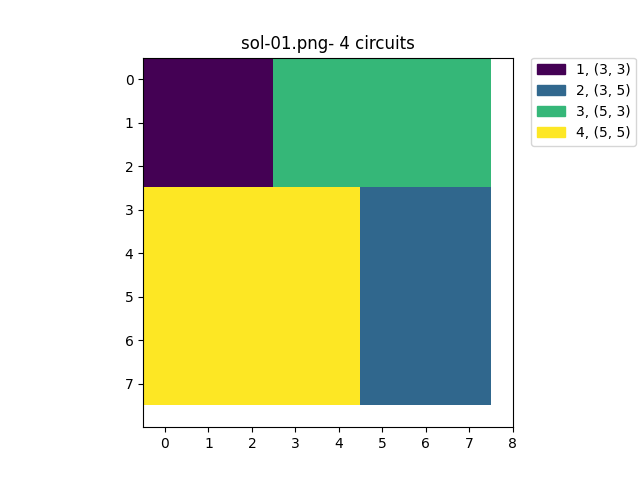
\includegraphics[width=12cm, height=10cm]{images/sol-01.png}
 \caption{Solution as image}
 \label{fig:future}
\end{figure}

\subsection{Final considerations}
By developing this project, many theoretical concepts are clarified and applied in a practical way. \\
As first step, we reasoned on how to model a problem identifying which are parameters and variables, how to encode it in different languages, such as Minizinc and SMT, then we tried to improve the model by introducing in Minizinc global constraints, implied constraints or conditions, and finally symmetry breaking constraints. We though that this procedure is much efficient. \\
Then, we did different experiments by changing configuration parameters, for Minizinc models, we found that the fastest way to find the correct solution is to apply \emph{first\_fail} as the criteria to choose the variable, and \emph{indomain\_min} to choose the value.\\

We can say that \textbf{CSP 1.3.0} seems to perform better than \textbf{SMT} and \textbf{CSP 1.0.0}, at least it should asymptotically do so. Below we have summarized some datum about the model mentioned on the \textbf{40} instances given as reference:
\begin{itemize}
    \item \textbf{Solved instances}: \textit{26};
    \item \textbf{Average solving time}: \textit{17.48s};
    \item \textbf{Total execution time for the solved instances}: \textit{454.53s}
\end{itemize}
\clearpage
	\nocite{*} % Flag to put all citations in the bibliography
	\printbibliography
\end{document}
